% !TEX program = xelatex
% Copyright 2026 Chen Jiaqi (GitHub: @H15teve)
% Distributed under LPPL 1.3c or later; maintenance status: maintained.
% Current Maintainer: Chen Jiaqi (GitHub: @H15teve).
% This work consists of the files listed in LPPL-MANIFEST.txt.
%==================================================================
%  golden-demo.tex — 中国电机工程学报 Word 模板逐字金样
%  内容与 Word 原文逐段一致,用于视觉回归验收
%  编译: xelatex golden-demo.tex (×3,无 biber)
%  参考文献: 手写 \cseebibliography 环境
%==================================================================
\documentclass[UTF8,twoside,a4paper,fontset=none]{ctexart}
% 金样回归必须锁定 Windows 原模板字体；跨平台写作请使用 paper-example.tex。
\usepackage[fontset=windows]{csee}
\graphicspath{{figures/}}

\cseeheader{中国电机工程学报}{Proceedings of the CSEE}

\begin{document}
\raggedbottom

%================ 篇首通栏题头 =================
\twocolumn[
% 原始 Word 模板的篇首教学注释块（金样逐字保留；正式写作接口见 paper-example.tex）
\vspace*{8.5pt}
{\fontsize{9pt}{16.2pt}\selectfont\songti
 \noindent\makebox[0pt][l]{\scalebox{0.9598}[1]{文章编号、中图分类号、文献标志码及学科分类号：中间标点为全角，字号小五号，中文黑体，数字及英文{\cseetnr Times New Roman}，}}\par
 \noindent\hspace*{5.086bp}\makebox[0pt][l]{（各项目之间空4格，中图分类号的英文字母与数字间留1/4字符空格）}\par}

% 中文标题（22pt 字号、36pt 行距）
% TeX 段落本身已形成 Word“段前 12pt”的可见效果；不再重复叠加空白。
% 注释块末行到标题的可见字框间距约为 15.20pt。
\vspace{8.7pt}
{\centering\heiti\sffamily\fontsize{22pt}{32.4pt}\selectfont 标题二号，黑体，英文字体为 Arial，希腊字母保\\持不变，如$\theta\omega_{\rho}\omega\Delta$，段前空 12pt\par}
\vspace{10.7pt}

% 作者(四号仿宋)
{\centering\fangsong\sihao 作者姓名四号仿宋，中间全角逗号隔开\par}
\vspace{6.83pt}

% 单位(五号楷体,两行)
{\centering\kaishu\wuhao（1．作者单位、地址五号楷体，标点均为全角）\\空一行，格式同上行\par}

% 英文标题（补偿上方三组间距后保持 Word 锚点）
\vspace{16.94pt}
{\centering\cseetnr\xiaosi\bfseries 英文标题小四号 Times New Roman加黑，实词和 4个字母及以上的虚词首字母大写(如\\With)\par}

% 英文作者(五号TNR)
{\centering\cseetnr\wuhao 英文姓名五号 Times New Roman，标点半角，姓大写，名首字母大写两字之间用连字符连接\par}

% 英文单位(小五TNR)
{\centering\cseetnr\xiaowu (英文单位小五号 Times New Roman，标点半角，实词首字母大写，虚词小写，段后空 12pt)\par}

% 以上部分行距段
{\xiaowu\songti 以上部分行距均为单倍行距，“如果定义了文档网格，则与网格对齐”“根据页面设置确定行高线”选项选中\par}
\vspace{20pt}
]% <— 通栏方括号在此闭合
\thispagestyle{csee-first}

% 在首页左栏开始处登记基金块；TeX 按实际内容高度为其预留栏底空间。
\cseefund{国家重点基础研究发展计划项目(973计划)\linebreak(2006CB200303，2006CB2003056)}{The National Basic Research Program (973 Program) (2006CB2003\cseefundbreak 03, 2006CB2003056).}

%================ 双栏正文(ABSTRACT 是闭合后第一段) =================
\begin{cseeabstractEN}
英文摘要为小五号 Times New Roman 字体，行距为 14pt，标点为半角。
\end{cseeabstractEN}
\cseekeywordsEN{英文关键词为小五号 Times New Roman 字体，{\cseesongbold 小写}，行距为14pt，中间标点为半角，段首空6pt}

\begin{cseeabstract}
中文摘要为小五号宋体，行距为14pt，中间标点为全角，段首空6pt。
\end{cseeabstract}
\cseekeywords{中文关键词为小五号宋体，行距为14pt，中间标点为全角，段首空6pt}

\section{二级标题为小四黑，英文字体为Arial，换行时悬挂缩进为0，段前段后均空6pt，希腊字母保持不变，如$\theta\omega_{\rho}\omega\Delta$}
正文字号五号，首行缩进 0.74cm，中文宋体，英文及数字为 Times New Roman，行距为单倍行距（“根据页面设置确定行高线”选项选中），段尾不要单字成行。文中字母与公式中字母应一样，文中括弧除列项说明为全角外，其余均为半角。

\subsection{三级标题五号黑体，英文及数字用Arial，希腊字母保持不变，如$\theta\omega_{\rho}\omega\Delta$。换行时悬挂缩进为0，段前段后不空}
\subsubsection{四级标题五号宋体，英文及数字用Times New Roman 字体，换行时悬挂缩进为0，段前段后}
\newpage
\noindent 不空\par

文中列项说明格式如下：

1）工作模式1。

2）工作模式2。

\subsubsection{数字的排版}
数字之间，自小数点起，前后每隔 3 位留 1/4 字符空格，数字和单位之间留 1/4 字符空格。如：12\,345.879\,08\,$\mu$m。正文中参考文献的序号和数字后的单位不能置于行首。

\subsubsection{文中标题的自动编号}
文中{\cseesongbold 标题为自动编号。标题的设计方法}是：将光标移至需要成为标题的段落中，通过按"Shift+Alt"和"←"或"→"（左箭头键或右箭头键），来设计1 级标题，或2 级、3 级等标题。方框下面给出的标题和编号是样板。

\subsubsection{正文的输入}
{\cseesongbold 正文的输入}，只需在标题输入完毕后，按回车键，即可直接输入；或者从“格式工具栏”

\vspace{15pt}
\noindent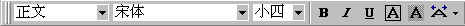
\includegraphics[width=7.541cm,height=0.556cm,keepaspectratio]{fig-toolbar1.jpg}的\par

\vspace{15pt}
\noindent
\includegraphics[width=2.369cm,height=0.556cm,keepaspectratio]{fig-toolbar2.jpg}中选择“正文”样式。\par

\vspace{3pt}
\subsubsection{图、表、参考文献、公式的编号}
文中的{\cseesongbold 图、表、参考文献、公式}一律采用阿拉伯数字单独连续编号。如图 1，表 2 或式(3)。如"图3 中国 1985—1990 年人口变化趋势图"就是指本论文的第 3 个图。建议采用全篇统一按原文中出现的先后顺序编码。附录中的{\cseesongbold 图、表、公式}另行编号，如图 A1，表B2（表示附录 B 中的第2 个表）。

\subsubsection{其他要求}
\subsubsection*{定义 1}

\subsubsection*{定理 1 （文字黑体顶格，数字 Times New Roman，加黑。）}

\subsection{变量和单位的要求}
文中所用的{\cseesongbold 变量和单位}一律采用国家标准，可参见国家标准《量和单位》（GB3100$\sim$3102-93）。每个变量的大小写、上下标等要全文统一，切勿混淆；每个变量符号只能用一个字符(可另加上、下标)表示，切勿用英文单词的缩写(字母组合)表示．相同的符号只能代表同一意义。

正文中如出现如下符号：$\cong\ \Phi\ \Gamma\ \vartheta\ \varsigma\ \Omega\ \alpha\ \beta\ \chi\ \delta\ \varepsilon$ $\phi\ \gamma\ \eta\ \iota\ \varphi\ \kappa\ \lambda\ \mu\ \nu\ \pi\ \theta\ \sigma\ \tau\ \varpi\ \omega\ \xi\ \psi\ \zeta\ \infty\ \times\ \pm\ +\ -$，请使用 Symbol 字体。

\subsection{公式的输入要求}
使用 MathType 公式编辑器。尺寸定义：完全10.5pt、上标/下标 6.5pt、次上标/下标 4.5pt、符号15pt、次符号 12pt；有编号的公式右对齐。公式 1行排不下时第 2 行以下应有明显缩进，公式转行时就优先在 $=$，$>$，$<$，$\rightarrow$ 等关系符号处，其次在\linebreak $+$，$-$，$\times$，$\div$，$/$ 等运算符号处转行；转行时关系符号和运算符号应位于上行末，下行首不再重复。\linebreak 对于“$\dfrac{a}{bc}$”类型的公式，改成横排时，不要排成“$a/b*c$”应改为“$a/(bc)$”，公式转行时排列格式如下：
\begin{equation}
\label{eq:1}
\begin{aligned}
\frac{I(h)}{I_{s}} = \frac{1}{h \pi} \left\{\frac{\sin [(h - 1)(\alpha + \pi / 2)]}{h - 1} - \right. \\
\left. \frac{\sin [(h + 1)(\alpha + \pi / 2)]}{h + 1} \right\} \frac{U_{m}}{U_{s}}
\end{aligned}
\end{equation}

% Word 金样中的 MathType 对象占用一个额外文档网格行。
\vspace{16.15pt}
\subsection{表格的要求}
1）中文表题小五黑，数字与英文字体及英文表题为 Times New Roman（加黑），居中，段前及英文表题后空 3 pt，行距为固定值 14 磅。

2）表中物理量：单位用分数形式表示，单位与物理量需折行排时，分数线要划在上一行的行末。

以百分数表示的量，一般用"$\varphi_{B}/\%$"表示。

3）表内栏目线 0.5pt，顶线和底线 0.75pt。表中文字为六宋，数字及英文为 Times New Roman，行距为 14pt。列间一律用制表位对齐。

% “示例”段前还保留一个文档网格行，用来复现原 Word 对象锚点。
\vspace{16.15pt}
示例：

\begin{cseetableblock}
  \cseetabletext
  \captionof{table}{\heiti 表\thetable\quad DPMA 与 DFT 算法的性能比较\\\cseetnr\bfseries Tab.\thetable\quad Performance comparison between\\DPMA and DFT algorithm}\label{tab:1}
  \begin{tabular*}{\linewidth}{@{\extracolsep{\fill}}ccccc@{}}
    \toprule
    算法 & $f_{\text{sp}}/\text{Hz}$ & $e_{\text{ang}}/(\degree)$ & $e_{\text{mag}}/\text{‰}$ & $e_{\text{TVE}}/\%$ \\
    \midrule
    \multirow{3}{*}{DFT}  & 2 & 0.099\,7 & 2.195\,9 & 9.971\,6 \\
                          & 3 & 0.148\,6 & 3.694\,5 & 14.863\,3 \\
                          & 4 & 0.194\,3 & 5.553\,8 & 19.521\,4 \\
    \midrule
    \multirow{3}{*}{DPMA} & 2 & 0.007\,3 & 1.241\,0 & 1.238\,1 \\
                         & 3 & 0.017\,3 & 2.771\,7 & 2.775\,1 \\
                         & 4 & 0.031\,5 & 4.884\,2 & 4.906\,5 \\
    \bottomrule
  \end{tabular*}
\end{cseetableblock}

\subsection{图的要求}
1）图的插入方式用"Word图片"，锁在文字中，居中，图中中文文字为六宋，英文字母为 {\cseetnr\bfseries Times New Roman} 体。图中线条的粗细要区分出主线和副线，主线用较粗的线 0.75 磅，副线用较细的线 0.5 磅。在曲线图中，数据曲线是主线，坐标线和指引线是副线；在流程图中，物注解线是主线，装置设备线是副线，设备结构图中，设备边框是主线，中心线，剖面线，尺寸线是副线。图形段前段后空 3pt。一般图形的标注见附录 A。

2）图题与表题相同，居中，中文为小五黑，数字与英文字体为 Times New Roman，加黑，行距为固定值 14 磅。英文图题段后空 3pt。

\subsection{论文中符号和缩略词的要求}
符号和缩略词在第一次出现时一一加以说明，给以明确的定义。示例：

{\songti 集成门极换向晶闸管 }{\cseetnr(integrated gate-commutated thyristor}{\songti ，}{\cseetnr IGCT)}{\songti 。}

\cseeacknowledgment{本文中实验方案的制定和实验数据的测量记录工作是在×××集团有限公司×××、×××、×××等工作人员的大力支持下完成的，在此向他(她)们表示衷心的感谢。}

%================ 参考文献区(手写 cseebibliography) =================
\begin{cseebibliography}
\item 葛俊，童陆园，耿俊成，等．TCSC暂态过程中晶闸管导通角特性的研究[J]．电网技术，2001，25(7)：18-22．\\
Ge Jun，Tong Luyuan，Geng Juncheng，et al．Research on thyristor conduction angle characteristics in transient process of TCSC[J]．Power System Technology，2001，25(7)：18-22(in Chinese)．\\
中文期刊：注：其中，“2001”为出版年，“25”为卷号，“7”为期号，“18-22”为起止页码；
\item 张贤达．现代信号处理[M]．北京：清华大学出版社，2002：179-193．
\item 昂温 G，昂温 P S．外国出版史[M]．陈生铮，译．北京：中国书籍出版社，1998：112-147．
\item Anderson P M，Agrawal B L，Van Ness J E．Subsynchronous resonance in power system[M]．New York：IEEE Press，1990：35-68．\\
中文专著：著作者．专著名称[M]．出版地：出版社，出版年：引用页码．
\item 袁慧梅．用 GA 优化的 ANN 在配电网线损中的应用[D]．北京：中国农业大学，1999．\\
学位论文：论文作者．论文名称[M]．学校所在地：学校名称，年度．
\item 蒋卫平．西北 750kV 系统电磁暂态实时仿真研究[R]．北京：中国电力科学研究院，2002．\\
报告：报告作者．报告名称[R]．报告单位所在地：报告存放单位，年度．
\item Sharma C．Modeling of an island grid[J]．IEEE Trans on Power Systems，1998，13(3)：971-978．\\
外文期刊：注意不要使用缩写的外文期刊名称，请给出全称。注：“Modeling of an island grid”为文章名称，“IEEE Trans on Power Systems”为期刊名，“1998”为出版年，“13”为卷号，“3”为期号，“971-978”为起止页码。作者的姓在前，名的首字母放在其后。
\item Kennedy J，Eberhart R．Particle swarm optimization[C]．Proceedings of IEEE Conference on Neural Networks，Perth，Australia，1995．\\
外国会议论文：作者．所参考的文章[C]．会议名称或者会议论文集名称，会议举办的城市，举办年度．
\item 全国文献工作标准化技术委员会第七分委会．GB/T 5795-1986 中国标准书号[S]．北京：中国标准出版社，1986．\\
标准：注：“全国文献工作标准化技术委员会第七分委会”为标准的制定者，“GB/T 5795-1986”为标准编号，“中国标准书号”为标准名称，“中国标准出版社”为标准的出版单位，“北京”为标准的出版地，“1986”为标准出版年。
\item 刘振亚．落实科学发展观加快建设坚强的国家电网[N]．中国电力报，2005-02-24(1)．\\
报纸：注：“刘振亚”为作者，“2005”为发表年，“02”为发表月，“24”为发表日，“(1)”为第1版。
\item PACS-L：the public-access computer system forum[EB/OL]．Houston，Tex：University of Houston Libraries，1989[1995-05-17]．\url{http://info.lib.uh.edu/pacsl.html}．\\
电子文献：著者．题名[文献类型标志/文献载体标志]．出版地：出版者，出版年（更新或修改日期）[引用日期]．获取和访问路径．
\end{cseebibliography}

%================ 附录 A =================
\vspace{21.4pt}% 补偿 Word 中电子文献说明多占的右栏网格行
\cseeappendixhead[A]
\renewcommand{\thefigure}{A\arabic{figure}}
\setcounter{figure}{0}
\renewcommand{\thetable}{A\arabic{table}}
\setcounter{table}{0}
\xiaowu\songti 附录是作为论文主体的补充项目，并不是必需的。\par

\noindent 附录格式：中文摘要为小五号宋体，行距为14pt。\par

\noindent 本刊要求的图形模式如下：\par

1）简单函数图。横纵坐标的标目（说明坐标轴物理意义的必要项目）应与被标注的坐标轴平行，居中排印在坐标轴与标值的外侧。标值应防止标注得过分密集，以至于数码前后连接，辨识不清。如图A1所示。

\begin{cseefigureblock}
  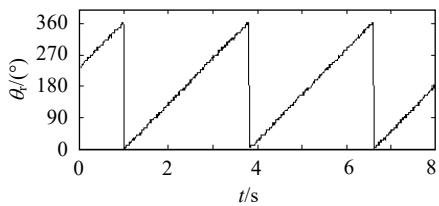
\includegraphics[width=5.715cm,height=2.540cm,keepaspectratio]{figA1.jpg}
  \cseefigurecaptionof{横/纵坐标有单位的简单函数图形}{Diagram of function curve in which x-axis and y-axis have unit}\label{fig:A1}
\end{cseefigureblock}

2）非定量的、且只有 1 个字母标注的简单标目，如 x,y 也可以直接地放在坐标轴顶端的外侧。如图A2所示。

\begin{cseefigureblock}
  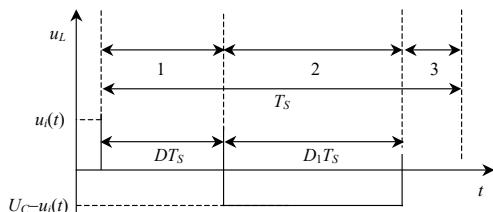
\includegraphics[width=6.285cm,height=2.725cm,keepaspectratio]{figA2.jpg}
  \cseefigurecaptionof{横/纵坐标为非定量的、简单标目的函数图形}{Diagram of function curve in which x-axis and y-axis haven't unit}\label{fig:A2}
\end{cseefigureblock}

3）录波图形的标准画法。录波图需标注横/纵坐标的物理量及每单元格所代表的数值及单位。如图A3所示。

\begin{cseefigureblock}
  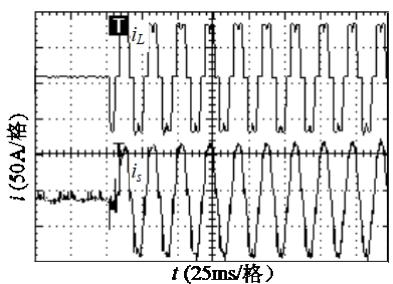
\includegraphics[width=5.212cm,height=3.598cm,keepaspectratio]{figA3.jpg}
  \cseefigurecaptionof{录波图形的标准画法}{Diagram from oscillograph}\label{fig:A3}
\end{cseefigureblock}

\cseebiographyintro{{\heiti 作者简介：}中文小五宋，数字及英文为 Times New Roman。行距14pt，首行缩进0.63cm，标点除括弧为半角外，其余均为全角。

文章第一作者须刊登照片，其余作者若全部提供照片，也予刊登，但若其中有作者不愿提供，则只刊登第一作者照片。照片应为近期数码证件照（不低于260$\times$330像素），宽2.2cm，长2.8cm。浅色背景，要求图像清晰，头部宽度（或高度）占照片宽度（或高度）的2/3，位置适中。}

\cseeauthorbio[\#\#\#]{author_photo.jpg}{(1974)，女，工学硕士，工程师，主要从事高电压试验技术、绝缘子检测和外绝缘方面的研究工作；12345678@126.com；}

% Word 第4页的作者简介多占一行；相应缩短照片与责任编辑之间的一行间距。
\vspace{-1.80pt}
\cseeeditor{李小丫}
\cseeeditornote{\mbox{五号黑体，\kern-0.36pt 编辑姓名楷体居右，\kern-0.36pt 段前空}\linebreak 6pt}

\raggedend\newpage
\begin{cseegeneral}
总则：\par
排版软件：Word 2007\par
页面设置：\par
整篇文档\par
纸张大小 A4，\par
页边距：上 3.2cm，下 2.5cm，左 2.0cm，右 2.0cm，栏间距 0.78cm，页眉 2.0cm，页脚 0\par
指定每页行数 42 行，每行字数 45（半栏 21）\par
整篇文档行距为单倍行距（"如果定义了文档网格，则与网格对齐"选项选中），字体五号宋体，英文五号 Times New Roman\par
篇首通栏部分为单倍行距，"如果定义了文档网格，则与网格对齐"项选中。\par
页眉小五号宋体，英文字体为 Times New Roman 用制表位对齐，第一制表位居中，8.5cm，第二制表位居右，16.8cm\par
\end{cseegeneral}

\end{document}
